\documentclass[10pt,executivepaper]{article}
\usepackage[utf8]{inputenc}
\usepackage[spanish]{babel}
\usepackage{amsmath}
\usepackage{amsfonts}
\usepackage{amssymb}
\usepackage{graphics}
\usepackage{graphicx}
\usepackage[left=2cm,right=2cm,top=2cm,bottom=2cm]{geometry}
\usepackage{imakeidx}
\makeindex[columns=3, title=Alphabetical Index, intoc]
\usepackage{listings}
\usepackage{xcolor}
\usepackage{multicol}
\usepackage{changepage}
\usepackage{float}
\usepackage{cite}
\usepackage{url}

\definecolor{codegreen}{rgb}{0,0.6,0}
\definecolor{codegray}{rgb}{0.5,0.5,0.5}
\definecolor{codepurple}{rgb}{0.58,0,0.82}
\definecolor{backcolour}{rgb}{0.95,0.95,0.92}

\lstdefinestyle{mystyle}{
    backgroundcolor=\color{backcolour},
    commentstyle=\color{codegreen},
    keywordstyle=\color{magenta},
    numberstyle=\tiny\color{codegray},
    stringstyle=\color{codepurple},
    basicstyle=\ttfamily\footnotesize,
    breakatwhitespace=false,
    breaklines=true,
    captionpos=b,
    keepspaces=true,
    numbers=left,
    numbersep=5pt,
    showspaces=false,
    showstringspaces=false,
    showtabs=false,
    tabsize=3
}

\lstset{style=mystyle}

\title{Algorithm}

\author{A cargo del profesor: Cristhian Avila Sanchez\\Escrito por: Adrian González Pardo}

\date{\today}

\newcommand\tab[1][1cm]{\hspace*{#1}}

\begin{document}
% Portada
%encabezado
\begin{minipage}{0.4\textwidth}
	\begin{flushleft}
		
\includegraphics[scale = 0.05]{logoescom.png}
	\end{flushleft}
\end{minipage}
\begin{minipage}{0.51\textwidth}
	\begin{flushright}
		
\includegraphics[scale = 0.055]{logoipn.png}
	\end{flushright}
\end{minipage}
\begin{center}
	\par\vspace{0.5cm}{
		\huge\textbf{Instituto Politécnico Nacional \\*[0.20cm] Escuela Superior de Cómputo}
	}
	\par\vspace{1cm}{
		\large\textbf{
		{Análisis y Diseño de Algoritmos\\Profesor: Cristhian Avila Sanchez\\Grupo: 3CV3\\Adrian González Pardo\\Semestre: 20/01}}
	}
	\par\vspace{1cm}{
		\includegraphics[scale=0.2]{AnalysisOfAlgorithm.jpg}
	}
	\par\vspace{2cm}{
		Ultima fecha modificado: \today
	}
\end{center}

% Indice
\clearpage
\tableofcontents
\clearpage

%Contenido
\section{Incio}
\subsection{Presentación}
El fin de comprender el Análisis y Diseño de Algoritmos en la ingeniería, es con la tarea de poder resolver problemas en los que se pueda automatizar procesos con el uso del poder computable aun cuando estos pueden tener una mayor complejidad en la Automatización de dicho, por lo cual se abordaran problemas acorde a su tipo de clase de complejidad y se llevara un análisis en el que se planea llegar a una aproximación de solución o a su solución total.
\subsubsection{Prerequisitos de la materia (No estrictos)}
\begin{center}
	\begin{tabular}{|p{5.5cm}|p{5.5cm}|}
		\hline
		Lenguaje C (o de la familia de lenguajes C) &	 Teoría de la Computación \\
		\hline
		Probabilidad &  Variable Compleja \\
		\hline
		Matemáticas Discretas &  Análisis Vectorial \\
		\hline
		Algebra Lineal &  Calculo I,II \\
		\hline
		Ecuaciones Diferenciales & Física \\
		\hline
	\end{tabular}
	\\\vspace{2.5mm}
	\begin{tabular}{|p{13cm}|}
		\hline
		\textit{Nota: es necesario tener noción de estos topicos debido
		a ciertos temás en los que se puede abordar acorde a temas anteriormente
		vistos y por otro lado es necesario saber como trabaja a bajo nivel todo
		el proceso de calculo de complejidad temporal y espacial con uso de bajo recurso.}\\
		\hline
	\end{tabular}
\end{center}
\subsubsection{Topicos de la materia}
De acuerdo al plan estudios propuesto en la pagína de la ESCOM se abordaran los siguientes temas tomando de guía el temario y los temas propuestos por el profesor.
\begin{center}
	\begin{tabular}{|p{5.5cm}|p{5.5cm}|}
		\hline
		Problemas P & Heuristicas\\
		\hline
		Complejidad Computacional & Programación Dínamica \\
		\hline
		Algoritmos Aleatorios & NP-Completos \\
		\hline
		Divide y Venceras & NP-Dificiles\\
		\hline
		Espacios de Busquedad & No Computables \\
		\hline
	\end{tabular}
\end{center}
\subsubsection{Evaluación de la materia}
La materia para este semestre sera evaluada de acuerdo a los siguientes rubros.
 \renewcommand{\labelenumi}{\Roman{enumi}}
\begin{enumerate}

	\item Examen 70\%
	\item Lista de problemas 10\%
	\item Practicas 10\%
	\item Evaluación Practica 10\%
\end{enumerate}
\subsubsection{Libros que pueden ser de ayuda}
\begin{itemize}
	\item Algorithm Design - Kleinberg, Tardos
	\item The Nature of Computation - Christopher Moore
	\item Cormen
	\item Sipser
	\item Hopcroft
\end{itemize}
\section{Primer parcial}
\subsection{¿Qué es un Algoritmo?}
Entre las ideas comunes de los que es un algoritmo estan:
\begin{center}
	\begin{tabular}{|p{11cm}|}
		\hline
		Es una solución a un problema computacional mediante una Maquina de Turing que siempre se detiene (Llega a un estado de aceptación)\\
		\hline
		Es parecido a una receta: Recibe una Entrada y pasa a una Salida\\
		\hline
		Serie de pasos ordenados y estructurados\\
		\hline
		Se puede reutilizar para distintos problemas / con variantes\\
		\hline
	\end{tabular}
\end{center}
De acuerdo a unas aproximaciones formales podemos tener que un algoritmo es:
\begin{center}
	\begin{tabular}{|p{11cm}|}
		\hline
		Solución a un problema computacional mediante una Maquina de Turing que siempre se detiene (Llega aun estado de aceptación) durante el procesamiento, parte de un estado inicial y va avanzando a través de los estados del automata\\
		\hline
		Algoritmo / Automata puede reutilizarse en diversas instancias del problema computacional (reutilización de la logíca o modulo computacional)\\
		\hline
	\end{tabular}
\end{center}
Entonces con esto podemos plantear algo muy importante que es:
\subsubsection{Computación}
Podemos definirla como un proceso natural en el que se busca una representación de un comportamiento físico, que a su vez es representado por un modelo matemático en el que se piensa puede representar un proceso, un comportamiento natural o incluso en el que se puede mostrar algo parecido a la vida.
\\
De este modo un algoritmo acorde a esta idea debe ser:
\begin{itemize}
	\item Eficas: Que debe tener una resolución correcta
	\item Eficiente: Que debe ser capaz de realizarlo con recursos óptimos (Memoria / Procesamiento)
\end{itemize}
\subsection{Complejidad Computacional}
La complejidad computacional puede ser interpretada como la integración del número de recursos que utiliza un algoritmo para resolver un problema computacional.\\
Esta complejidad esta dividida en dos clases muy importantes:\\
\begin{itemize}
  \item Temporal: Con relación al procesamiento
  \item Espacial: Con relación a la memoria
\end{itemize}
De este modo podemos pensar y añadir a las caracteristicas de la resolución de un algoritmo:
\begin{itemize}
  \item Eficacia: A una correctez en su ejecución
  \item Eficiencia: A una buena administración de sus recursos (Memoria - Espacio) (Procesamiento - Tiempo)
\end{itemize}
\subsubsection{Enfoque temporal}
Ahora como una primera aproximación: Asumiendo un espacio utilizado constante o manejable.\\
\textbf{Definimos:}\\
Función temporal: \\
\tab $\mathbf{f(N)}$: Es el número de pasos / operaciones a ejecutar.\\
\tab $\mathbf{N}$: Es el numero de datos de entrada.\\
Acorde a esto podemos pensar en que existen complejidades:\\
\tab Lineal: \\\tab\tab$\mathbf{f(N) = kN; \tab k \in \mathbb{R}}$\\
\tab Cuadrática: \\\tab\tab$\mathbf{f(N)  \sim {N^2}}$\\
\tab Polinomial: \\\tab\tab$\mathbf{f(N) \sim {N^a}}; \tab a \in \mathbb{N}$\\
\tab\tab\textbf{$\mathbf{f(N) \sim \alpha{\scriptscriptstyle a}N^a + \alpha{\scriptscriptstyle a-1}N^{a-1} + ... + \alpha{\scriptscriptstyle 2}N^2 + \alpha{\scriptscriptstyle 1}N + \alpha{\scriptscriptstyle 0};\tab \forall\alpha{\scriptscriptstyle i} \in \mathbb{R}}$  \&  $ i \in [0 , a]$}\\
\tab Logaritmica: \\\tab\tab $\mathbf{f(N) \sim \log{N}}$\\
\begin{center}
  La idea de algunos enfoques temporales a nivel Logatirmicos pueden ser los \textit{algoritmos de ordenamiento}, que graficamente su comportamiento se puede ver así:
  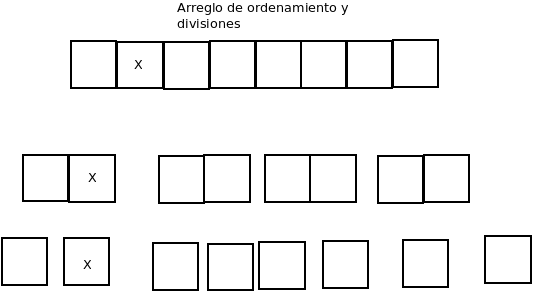
\includegraphics[scale=0.8]{draws/enfoqueTemporal1.png}\\
  \texttt{Figura 1}
  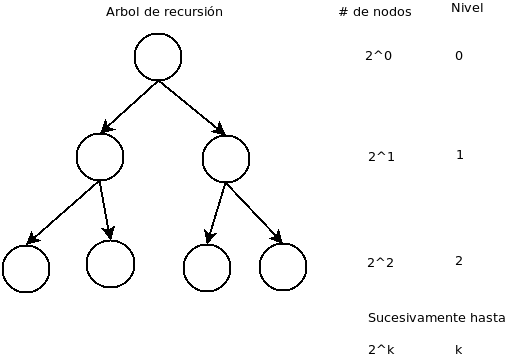
\includegraphics[scale=0.8]{draws/enfoqueTemporal.png}\\
  \texttt{Figura 2}
\end{center}
De este modo llevando un analisis de la Figura 1 y 2 que estan relacionadas podemos decir que si se suman los elementos que existen por nivel tomando un valor discreto $N$ siempre sumara $N$ no importando el nivel por lo tanto de acuerdo al número de nodos que existe $2^k$ tal que $k \notin Z^-$ podemos decir que $k= log_2{N}$ \\\tab$\therefore 2^k = N$
\subsubsection{Ordenamiento [Introducción a clase Polinomial (P)]}
De este modo podemos dar una pequeña introducción a los algoritmos de ordenamiento.\\
Sabemos que existen algoritmos que trabajan con una coleccion de datos de un solo tipo [llamese estruturas de datos, clases (caso de que se este usando el paradigma Orientado a Objetos) o variables] por lo que en algunas ocasiones es necesario realizar un ordenamiento a estos datos, por lo que se puede pensar en los algoritmos que sean sencillos de entender, por lo que más adelante algunos seran explicados a fondo de como trabajan y como se implementan a nivel pseudocodigo, por otro lado ya que se menciono acerca de complejidades temporales los algoritmos son:
\begin{itemize}
  \item Bubble sort: $N^2$
  \item Selection sort: $N^2$
  \item Merge sort: $N log N$
  \item Heap sort: $N log N$
  \item Quick sort: $N log N$
  \item Aleatorio: $f(N)$ donde $f$ es una función que puede ser representada como ecuación lineal, diferencial o de densidad probabilistica.
\end{itemize}
\subsubsection{Algunos otros algoritmos e ideas de problemas de la Clase NP}
Si bien sabemos que a nivel computacional podemos almacenar conjuntos de bits (0 vs 1) si lo vemos asociado a direcciones de memoria o variables con capacidad de $N$ bits podemos partir de que existe una complejidad de dar con la combinación de esos $N$ bits de $f(N)=2^N$ \\
Tomando ciertas ideas de esta notación de complejidad de $f$ podemos pensar en Grafos \\$\therefore$ Sea un Grafo $G=(V,E)$ \\Donde:\\
\tab $V=$ Es el conjunto de Vertices o nodos que existen
\\\tab $E=$ Es el conjunto de Aristas que se relacionan con los vertices\\
Si pensamos que $G$ es completo (Es decir que cumple un modelo combinatorio)\\
\tab\tab$|E|=\begin{pmatrix}
  N\\2
\end{pmatrix} = \frac{N!}{2(N-2)!} = \frac{N(N-1)}{2} = M$\tab$(0)$\\
\tab\ Donde:
\\\tab $N=|V|$\tab$(1)$\\
\\Sustituyendo 1 en 0 podemos tomar la idea y el formalismo matemático siguiente:\\
\tab $|E|=\begin{pmatrix}
  |V|\\2
\end{pmatrix} = \frac{|V|!}{2(|V|-2)!} = \frac{|V| ( |V|-1 )}{2} = M $\tab$(3)$\\
\begin{center}
  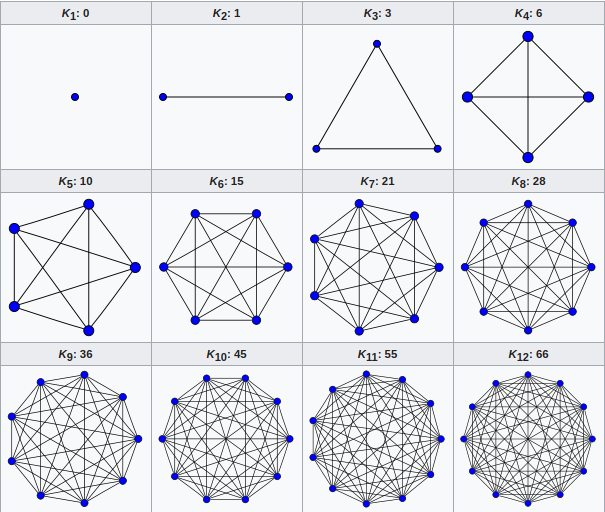
\includegraphics[scale=0.5]{images/grafoCompleto.png}\\
  \texttt{Figura de $G$ desde $N=1$ hasta $N=12$ vertices\\Cumpliendo 3}
\end{center}
Ahora imaginemos el que pasaria si buscamos explorar o asemejar un Grafo completo $G$ que va en crecimiento sucesivamente, es obvio que el hecho de ver el modelo combinatorio de $G$ y de sus caracteristicas el hacerlo es más difícil aproximarlo a un análisis Polinomial, lo cual podemos dar una pequeña introducción a la clase de problemas No Polinomiales (NP)
\subsubsection{Complejidades en NP vs P}
Si bien sabemos que esta complejidad representa un espacio combinatorio o exponencial algunos autores suelen expresar sus funciones de la siguiente forma.
\begin{center}
  \begin{tabular}{ p{5cm} p{4cm} }
    Complejidad Combinatorial & $f(N,K)=\begin{pmatrix}N\\K\end{pmatrix}$\\
    Complejidad Exponencial & $f(N,b)=b^N$\\
  \end{tabular}
\end{center}
Una vez que tenemos idea de este tipo de clases de complejidad podemos pensar que pueda existir un Lema, Teorema o Transformación, en la que se pueda decir que los problemas de clase P estan contenidos o no en los problemas de clase NP $P \subseteq NP $ o $P \nsubseteq NP$ lo cual es uno de los tantos problemas que existe de \textbf{Clay Institute of Mathematics $P vs NP$}\\
Si partimos de esta idea y de lo que se intenta hacer en las ciencias de la computación podemos pensar que generalmente o implicitamente la computación busca la automatización u otro fin en el que su participación ayude a desarrollar algo del día a día por lo cual podemos pensar que la clasificación NP, es la que engloba estos problemas y conjunto de soluciones, en los que si pensamos a traves de formalismos ya existentes podemos decir que estos problemas son mapeados a cuestiones de Computación, Matemáticas y Física, lo cual puede representar un isomorfismo o transformación de ir de un tipo de solución a otra.\\
Esto pensando en la definición de lo qué es un algoritmo la cual representa una máquinaria en la que representa lenguajes y leyes de un universo, pensando en esto podemos hablar de un cientifico que logro llegar a una idea de Maquina Universal que Teorícamente abordo el matemático Alan Turing y Alonzo Church, que es la $maquina$ $Z$ de Konrad Zuse quien realmente es el padre de la computación
\subsubsection{Maquina Z}
Si bien conocemos la historia de la Maquina de Turing fue famosa por el hecho de generar un procesamiento bajo unas reglas de su tupla, por lo que fue famosa por el hecho de que sus avances fueron pertenecientes a la segunda guerra mundial, pero esta otra maquina que es mencionada ya que esta maquinaria genera y sigue los principios de las computadoras actuales, en el cual esta maquina era programable a nivel de código binario y al igual que operaciones a bajo nivel de bits, esta maquina podia realizar operaciones binarias, para años en los que el modelo de Turing existia para la 2{\tiny da} guerra mundial, en esta maquina existia la Z{\tiny 3}, en la cual esta maquina realizaba operaciones aritmeticas, en la cual más tarde con su nuevo modelo Z{\tiny 4} lograba tener una aritmetica compleja, ahora que teniendo esto en cuenta podemos pensar acerca de \textbf{¿Qué representa un número complejo?}
\subsubsection{Número complejo}
Son aquellos números que complementan a sistemas de ecuaciones donde sus soluciones no son cubiertas al $100\%$ por el conjunto de números reales $\mathbb{R}$ por lo que se extiende el espacio del conjunto de números a los complejos, los cuales son representados de la forma $z=x+iy$ donde $x,y \in\mathbb{R}$, ahora en terminos de resoluciones aritmeticas que realiza una computadora, podemos pensar acerca de que en la computación a nivel físico estos numeros intervienen en la interacción con los componentes para la transmisión y realimentación de los chips, como tambien en algunos otros casos en donde se procesan señales de audio o señales de pixeles para el coloreo de pantallas o renderizado de imagenes.
\subsubsection{NP (Subclase NP-Completo)}

Dentro de los problemas que se pueden solucionar con estos conceptos y previas ideas de matematicas y algunas ideas implicitas de fenomenos físicos esta una subclase de los problemas NP, que son los problemas NP-Completos. Tales problemas que caen en esta clasificación son los siguientes:
\begin{center}
  \begin{tabular}{|p{5.5cm}|p{5.5cm}|}
    \hline
    Planificación & Optimización\\
    \hline
    Agrupamiento & Particionamiento\\
    \hline
    Redes & Teoría de Juegos\\
    \hline
    Circuito Hamiltoniano (Agente viajero) & Knaspsack (Max/Min)\\
    \hline
  \end{tabular}
\end{center}

\printindex
\end{document}
